\newcommand{\SScert}{SimSoC-Cert\xspace}

\section{Main Lines of SimSoC-Cert}
\label{sec:overallarchi}

\subsection{Overall Architecture}
The overall architecture of our system, called SimSoC-Cert, 
is given in Fig.~\ref{fig:archi}.
More specifically, we can see the data flow from
ARMv6 Reference Manual to the simulation code. 
Some patches are needed from the textual version of
the reference manual because the latter contains some minor bugs.
Three kinds of information are extracted for each ARM operation:
its binary encoding format, the corresponding assembly syntax
and its body, which is an algorithm operating on various
data structures representing the state of an ARM: registers, memory,
etc., according to the fields of the operation considered.
This algorithm may call general purpose functions defined
elsewhere in the manual,
for which we provide a Compcert-C library to be used by the simulator
and a Coq library defining their semantics.
The latter relies on Integers.v and Coqlib.v from CompCert library
which allows us, for instance, 
to manipulate 32-bits representations of words.
The result is a set of abstract syntax trees (AST) and binary
coding tables.
These ASTs follow the structure of the (not formally defined)
pseudo-code. 
Then two files are generated: 
a Coq file specifying the behavior of all operations
(using the aforementioned Coq library)
and a Compcert-C file to be linked with other
components of SimSoC (each instruction can also be executed
in standalone mode, for test purposes for instance).
More details are provided in \cite{rapido11}.



\begin{figure}
\hfil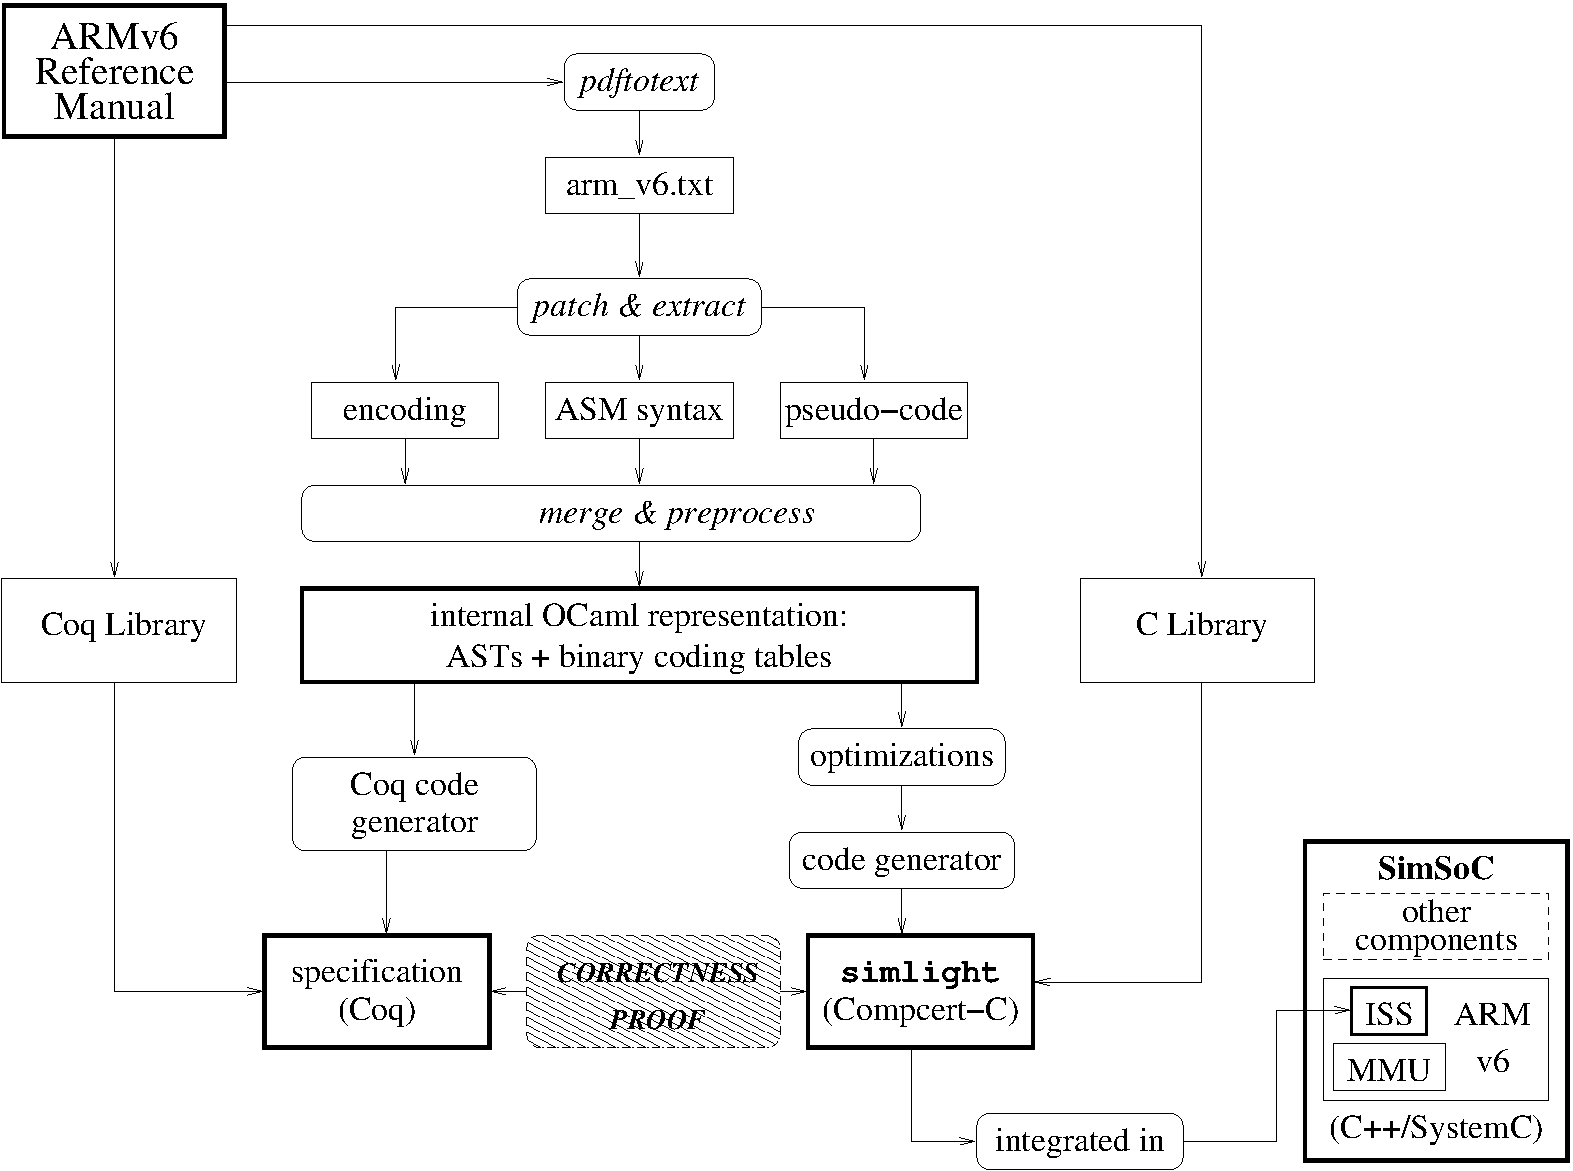
\includegraphics[width=.95\linewidth]{fullarchi.pdf}
\caption{Overall Architecture}
\label{fig:archi}
\end{figure}

The decoding of ARM operations is not considered in the present paper:
this is important and planned for future work,
but is less urgent since we were already able 
to automatize the generation of intensive tests,
as reported in \cite{rapido11}. 
We therefore focus first on the algorithmic body of operations.
In order to state their correctness,
we need Coq ASTs for the Compcert-C statements of \simlight.
The code generator directly generates such ASTs.
Another option would be to work on a generated textual (ASCII)
presentation of the Compcert-C code,
but we prefer to avoid additional (and possibly unreliable)
parsing step as far as possible.
We will see in Section \ref{sec:simlight}
that these ASTs are moreover presented in a readable form using
suitable notations and auxiliary definitions.

The whole \simlight project is currently well-compiled by
Compcert (targeting Intel code) and gcc; moreover validation tests
succeed completely with both simulators.
The version of \simlight compiled with Compcert can serve 
as a reference simulator,
but for most purposes the version compiled with gcc is prefered
for its higher speed.
% JF: commented out because of a remark from reviewer 2:
  % You suggest that staying within an "extensively tested" subset of C
  % means that using GCC is safe. Recent results from  Regehr et al. 
  % suggest otherwise. For example, GCC micompiled "(x / -1) != 1" to
  % "0". Perhaps your claim is true with optimizations turned off.
  % However, with no optimizations, GCC may actually be slower than
  % CompCert!
% Moreover, gcc is not that a bad choice as long as no exotic
% feature of C is used for \simlight,
% so that we stay in an extensively tested subset of C.

%% \todo{what about this paragraph in comment? :}
%% However, to use the main Compcert theorem, establishing the same
%% behavior of \simlight as the executable produced, it is required to
%% prove a not \emph{wrong behavior} of \simlight, by exhibiting one
%% constructively. Instead we think this task will be done implicitly at
%% the equivalence proof time. Then, we will have an equivalence to Coq,
%% and from Coq we know its behavior can not be \emph{wrong}. Remark that
%% even if this reasoning relies on classical logic, in the
%% intuitionistic one, we can anyway prove that later, our confidence increased by the equivalence proof.

%%%%%%%%%%%%%%%%%%%%%%%%%%%%%%%%%%%%%%%%%%%%%%%%%%%%%%%%%%%%%%%%%%%%%%

\subsection{Stating Correctness Theorems}

Let us now present the purpose of the gray box
of Fig.~\ref{fig:archi},
which represents our main target.

The correctness of simulated ARM operations is stated
with relation to the formal semantics of ARM
as defined by our Coq library and partly automatically produced
by the Coq code generator (the box called ``specification'' in
Fig.~\ref{fig:archi}).
Note that ARM operations are presented in a readable way using
suitable monadic constructs and notations:
apart from the security provided by automatic generation,
this greatly facilitates the comparison with the original pseudo-code
of the reference manual.
That said, it should be clear that the reference semantics
of ARM is the Coq code provided in these files.
Much effort has been spent in order to make them as clear
and simple as possible.

In contrast, the Coq description of the behavior of corresponding
operations (as simulated by SimSoC -- Compcert-C programs)
is far more complicated, though the superficial structure
is quite similar. This will be detailed in Section~\ref{sec:simlight}.
In particular, the memory model of the latter version is much more 
complex.
In order to state correctness theorems, we define a relation
between 
an ARM state represented by the Compcert-C memory model
and 
another ARM state, as defined by the Coq formal semantics.
Essentially, we have a projection from the former to the latter.
Then for each ARM operation, we want a commutative diagram
schematized in Fig.~\ref{fig:thrm}.


\begin{figure}
\hfil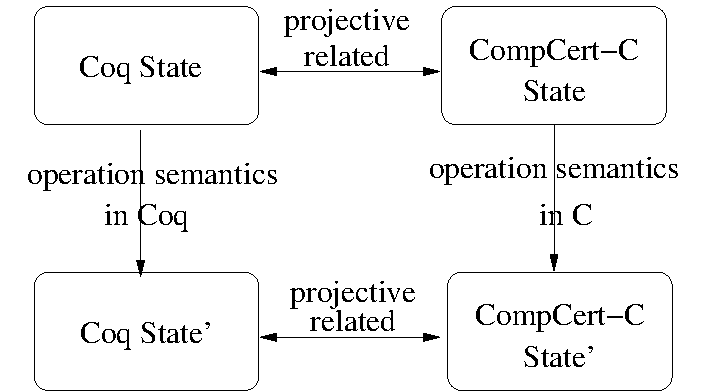
\includegraphics[width=.5\linewidth]{theorem_Coq2C.pdf}
\caption{Correctness of the simulation of an ARM operation}
\label{fig:thrm}
\end{figure}

For now, our automatic generation tools operate completely,
i.e., 
we have a Coq formal specification and a Compcert-C simulator 
for the full instruction set of ARM V6.
About proofs, 
the relationship between the abstract and the concrete memory models
is available;
we can then state correctness theorems for all ARM operations.
The work on correctness proofs themselves started recently.
We considered a significant ARM operation called \texttt{ADC}
(add with carry).
Our main theorem (Theorem 1 in Section \ref{sec:results})
states intuitevely that the diagram given
in Fig.~\ref{fig:thrm} commutes for \texttt{ADC}.
Its proof is completed up to some axioms on library functions,
details are given in Section~\ref{sec:results}.

%%% Local Variables: 
%%% mode: latex
%%% TeX-master: "cpp"
%%% End: 
